\section{Introduction}

Data collection processes proliferate due to the emergence of embedded
systems and sensor networks, providing opportunities to collect large
amounts of data.  These data should be analysed and processed by
information systems to be useful. A typical processing, for instance,
is to detect eventual sensor failures or malfunctions and, if it is
possible, to reconstruct the faulty data. The acquired data instances
hold a timestamp. Therefore, correctness criteria must include both
data values and their timestamps. The sequences of data values
collected at specific timestamps are formalised as \emph{time series}.

A time series is a collection of chronological observations.  In
general, we continously acquire a time series from phenomena
monitoring. On the one hand, we can record observations at regular
intervals, such as hourly or daily ones, resulting in equally spaced
time data.  On the other hand, we can record observations at irregular
intervals, such as recording when a pump is open or closed, resulting
in unequally spaced time data. Time series data are often voluminous
\cite{fu11,keogh08:isax}, thus efficiently storing and accessing them
can be complex. Moreover, this is especially critical when developing
small embedded systems with constrained resources (capacity, energy or
processing power) \cite{yaogehrke02}. Additionally, unequally spaced
time data increases the difficulty of processing.

The literature describes several attempts to build systems devoted to
managing and store time series data. These systems are generically
known as \emph{Time Series Data Base Management Systems}
(\acro{TSMS}), \cite{dreyer94,last01}. However, as shown below, most
of them exhibit some drawbacks when trying to solve the challenging
issues of time series in the temporal data domain.

Time series can be stored and managed by \emph{relational database
  management systems} that are usually queried using \emph{Structured
  Query Language} (\acro{SQL}). Nonetheless, some authors
\cite{dreyer94,schmidt95,stonebraker09:scidb,zhang11} notice that the
use of \acro{SQL} systems as a time series backend suffers from some
drawbacks.

\acro{NoSQL} or \acro{NewSQL} products are being developed to
increase the performance and flexibility of \acro{SQL} systems
\cite{atzeni13:relational_model_dead,stonebraker10,stonebraker09:scidb,zhang11}. It
is natural to consider them to store time series data. Indeed, the
continuous acquisition nature of the time series poses an issue when
trying to store and analyse all the data \cite{keogh97}.

We can apply compression techniques in two distinct styles to face the
challenges posed by time series data. First, to get an approximation
to the original signal that facilitates to do pattern search analysis
or finding similarities\cite{fu11,keogh01,last01}. Second, as a
compression and aggregation approach that leverages the storage of
massive \emph{data streams}
\cite{cormode08:pods,bonnet01}. Nonetheless, handling time series like
data streams neither considers adequately the time dimension nor
computes the evolution of aggregated parameters along the time, which
is interesting for monitoring purposes.

\emph{RRDtool} \cite{rrdtool} is a system that stores time series
aggregated using different resolutions. These characteristics allow
to compact the data and facilitates faster visualisations. In spite of
this, because \emph{RRDtool} is a particular application,
aggregation operations are limited to network monitoring.


\subsection{Contributions}

This paper formalises a model for \acro{TSMS} that stores and manages
time series data. This model exhibits several unusual characteristics:

\begin{itemize}

\item It organises the data in an aggregated way and it allows to
  store time series using different time resolutions. We know this
  feature as \emph{multiresolution}.  Thus, being multiresolution the
  most salient characteristic of our model, we name the formalised
  system \emph{Multiresolution Time Series Data Base Management
    System} (\acro{MTSMS}).  The model is designed to satisfy the
  requirements of bounded storage computers such as sensor systems.

\item It is a \emph{lossy storage} solution. Multiresolution allows
  for a lossy storage solution that selects only the relevant data. In
  some sense, multiresolution is close to the lossy compression
  methods used in multimedia applications, that discard meaningless
  data in favour of size.

\item It considers the time sampling irregularities of time series and
  operates coherently with the time dimension of time series.

\item It offers a degree of genericity to cope with the semantic
  characteristics of the actual data.

  Multiresolution requires aggregating several data instances into a
  single one. We abstracted this through an \emph{aggregation
    function} bound to the precise semantics of the actual
  data. Because of this, aggregation functions are set as an
  independent object of the main model.  Users can define new
  aggregation methods better suited for particular fields.

  The model also formalises the concept of time series
  \emph{representation function}.  This concept allows users to define
  different operators considering the behaviour of time series in
  different contexts. This issue is important to manage the precise
  semantics of the stored time series.

\item It is soundly formalised using set algebra and, particularly,
  relational algebra.

\end{itemize}

Our model shares some of its characteristics with other known
approaches. The analysis of \emph{RRDtool}~\cite{rrdtool} inspired the
multiresolution. However, we provide a sound formalisation that lacks
in~\cite{rrdtool} and a degree of genericity unavailable in
\emph{RRDtool}. Based on this facility, in our model we can define
particular time series aggregations like those of\emph{RRDtool}. To
formalise time series we follow the same approach used to formalise
bitemporal data for a relational \acro{DBMS}. The model favours more
recent data over the older one, which is in common with some other
methods, like that of Cormode et al.~\cite{cormode08:pods}.

We remark that the only goal of the model formalised here is to manage
time series data. In practical applications, it would be usual to
complement this model with a standard database system to handle all
the remaining data if needed. For instance, time series metadata such
as units of values, sensor localization or classification tags would
be stored in a standard \acro{DBMS}.


\subsection{Outline}

This manuscript is organised as
follows. Section~\ref{sec:related-work} introduces previous work that
concerns \acro{TSMS} and \acro{MTSMS}.  The motivation for
multiresolution is set out in Section~\ref{sec:features}.  We describe
the model in two steps.  First, in Section~\ref{sec:model:TSMS} we
formalise a \acro{TSMS} model devoted to the basic elements and
operations of time series.  Second, in Section~\ref{sec:MTSMS} we
formalise a \acro{MTSMS} model that extends the previous one with
multiresolution capabilities.  In Section~\ref{sec:implementation} we
describe an implementation of the integrated \acro{TSMS} and
\acro{MTSMS} model. Section~\ref{sec:example} is devoted to a real
data multiresolution database example.  Finally,
Section~\ref{sec:concl-future-work} offers some conclusions.


\section{Previous work}
\label{sec:related-work}

For the sake of completeness here we describe some previous work
related to time series storage. We organise this in three
subsections. First, we introduce some previous approaches to database
management systems for time series. Second, we explain how some
authors applied compression techniques to leverage time series
storage. Third, we review time series storage systems based on the
data streams paradigm.


\subsection{Database approaches}

According to some authors, \acro{TSMS} should be considered as a
specialised relational \acro{DBMS}~\cite{last01}.  Segev and
Shoshani~\cite{segev87:sigmod} propose a structured language for
querying \acro{TSMS}. Their time series structures include the notion
of regularity and temporal representation and their operations are
\acro{SQL}-like.  Dreyer et al.~\cite{dreyer94} suggest the
requirements of a particular purpose \acro{TSMS} and base the model on
five basic structural elements: events, time series, groups, metadata
and time series basis. They implement a \acro{TSMS} named
\emph{Calanda} which includes calendar operations, it allows grouping
of time series, and it operates with simple queries. They exemplify it
using financial data. In~\cite{schmidt95} \emph{Calanda} is compared
with temporal systems designed for time series.
 
Other authors consider array database systems well suited to
\acro{TSMS}.  \emph{SciDB}~\cite{stonebraker09:scidb} and
\emph{SciQL}~\cite{zhang11} are array database systems intended for
science applications, in which time series play a principal role. They
structure time series into arrays to achieve multidimensional analysis
and they store other data into tables.  \emph{SciDB} is based on
arrays which, according to the authors, allow to represent time
series.  In contrast, \emph{SciQL} defines time series as a mixture of
array, set, and sequence properties and exhibits some managing
characteristics for time series that include dealing with regularities,
interpolation or correlation queries.

\emph{Bitemporal} \acro{DBMS}, sometimes referred directly as
\emph{temporal data}, is a database field that inherently considers
temporal dimension of data. Bitemporal data manages historical data
and events in databases by associating pairs of \emph{valid} and
\emph{transaction} time intervals to data.  Bitemporal data and time
series data are not exactly the same, and so they cannot be treated
interchangeably~\cite{schmidt95}, however, there are some similarities
that can be considered. \acro{DBMS} research represents bitemporal
data as relations extended with time intervals attributes and enlarge
relational operations to deal with time related
aspects~\cite{jensen99:temporaldata,date02:_tempor_data_relat_model}.


\subsection{Compression approaches}

Oetiker's \emph{RRDtool}~\cite{rrdtool,lisa98:oetiker} is a free
software database management system designed for monitoring
systems. Because of this, it is focused on a particular kind of data,
gauges and counters, and it lacks general time series
operations. \emph{RRDtool} can store data at diverse time
resolutions. Plonka et al.~\cite{lisa07:plonka} evaluated
\emph{RRDtool} performance and found limitations when storing a vast
number of different time series. They suggested a caching system on
top of \emph{RRDtool} as a solution. Weigel et al.~\cite{weigel10}
advocate for a similar approach that caches queries by aggregate
parameters.  In Weigel's paper, the authors state that other systems
only show subsets of data, but they also consider necessary to show
data in their complete time span. They developed the software package
known as \emph{TSDS} that fully stores time series and then query them
by date ranges or by applying different filters and operations to the
data.

Deri et al.~\cite{deri12:tsdb_compressed_database} suggested
\emph{Tsdb}, a lossless compression storage \acro{TSMS} for time
series that share the same time instants of acquisition. Different
series are stored grouped by the acquisition time instead of in an
isolated way.  Deri et al. compared \emph{Tsdb}, \emph{RRDtool}, and a
relational product. They found that as a consequence of its structure,
\emph{Tsdb} achieves a better measure store time but a worse measure
retrieval time than other products. The need to be continuously
regrouping data is the cause of the differences.  However, when
the measures share the same time, \emph{Tsdb} considers them as the
same time series and measure retrieval time improves. In these
circumstances, it would be interesting to use the \emph{Tsdb}
implementation architecture of shared time arrays in a \acro{MTSMS} to
achieve a better storage performance.

Some of the lossy compression techniques for time series pursuit an
optimal approximation representation. They seek to balance between the
least amount of data that can reconstruct the original signal and the
data that gives the least error. Keogh et al.~\cite{keogh01} cite some
possible approximation representations for time series such as Fourier
transforms, wavelets, symbolic mappings or piecewise linear
representation. They remark the last one as very usual due to its
simplicity and develop a system called
\emph{iSAX}~\cite{keogh08:isax,keogh10:isax} to analyze and index
massive collections of time series. They argue that the main problem
is the indexing of time series, and they propose some efficient
methods. The first method proposed is based on a constant piecewise
approximation. The time series representation obtained with
\emph{iSAX} allows to reduce the stored space and faster indexing
while maintaining the quality achieved by more sophisticated methods.
These compression techniques are candidates for being used as
attribute aggregate functions in the \acro{MTSMS} model.


\subsection{Data stream approaches}

\emph{Cougar}~\cite{bonnet01} is a sensor database system that
maintains two main structures: a relational structure for sensor
properties and a set of data sequences for time series coming from
sensors. \emph{Cougar} time series have specific operations that can
combine relations and sequences. \emph{Cougar} target field is sensor
networks, where data are stored distributed in different
locations. Queries in \emph{Cougar} are resolved by combining sensor
data in a data stream abstraction. According to the authors, this
improves the processing performance.

To compute statistical aggregates, some authors consider time series
as data streams. Cormode et al.~\cite{cormode08:pods} developed some
aggregation techniques that give more weight to recent data and that
allow to run fast approximate queries on compressed data.

Dou et al.~\cite{dou14:historic_queries_flash_storage} create index
structures as multiresolution aggregates, like average, count, or top,
for historical data managed in a flash storage. They consider a specific
storage solution based on a register with pointers similar to the
multiresolution storage in \emph{RRDtool}~\cite{lisa98:oetiker}.


\section{Multiresolution motivation}
\label{sec:features}

An important characteristic of the model formalised in this paper is
\emph{multiresolution}. In a previous work, we analysed the
requirements, and we summarised the main target for multiresolution
systems \cite{llusa13:aiked}.

In this section, we motivate the advantages of the multiresolution
approach. First, we intuitively introduce the concept of
multiresolution through an example. Then, we discuss the benefits of
this formulation.

Figure~\ref{fig:mtsms:sequence} shows an example of the
multiresolution approach. In the upper part, there is a representation
of a signal being monitored. The signal values range from $0$ to $10$
along the time. There are two specific time instants marked in the
figure:

\begin{enumerate}

\item The first, marked with the word \emph{init}. It refers to the
  instant when the database started to receive signal samples.

\item The second, marked with the word \emph{now}. It refers to the
  instant when the process made the snapshot.

\end{enumerate}

Note that time coordinates are assumed to be positive for the time
instants after \emph{init} and negative otherwise. The time before
\emph{now} corresponds to the past and the time after \emph{now} to
the future.  The data before \emph{init} are unknown to the database.

\begin{figure}
  \centering
  %\tikzsetnextfilename{fig_mtsms_sequence}
  %%\usetikzlibrary{positioning}
\begin{tikzpicture}[scale=0.77, every node/.style={transform shape}]

  %referencia
  \node (-6) {};

  \foreach \x in {-5,...,12}
  {
    \pgfkeys{/pgf/number format/.cd,int trunc}
    \pgfmathparse{abs(\x)}
    \let\absx=\pgfmathresult
    \pgfmathparse{\x-1}
    \let\antx=\pgfmathresult
    %time
    \node[node distance=1mm] (\x) [right=of \antx] 
    {\ifnum\x<11 \x \else \phantom{9} \fi};

    %graph values
    \node [above=\absx mm of \x] 
    {\ifnum\x=10 \color{gray} \fi \ifnum\x<11 $\bullet$ \fi};    

    %values
    % \node[rectangle,draw] (s\x) [below=of \x] 
    % {\ifnum\x<10 \pgfmathprintnumber{\absx} \else \phantom{9} \fi};
    \ifnum\x<10
    \node[rectangle,draw] (s\x) [below=of \x] 
    {\pgfmathprintnumber{\absx}};
    \else
    \node[rectangle,dotted,draw] (s\x) [below=of \x] 
    {\phantom{9}};
    \fi
  }

  \node [below=of 10] {\color{gray}10}; 
  

  
  %rd: 5s |inf| mean
  \node [circle,draw] (rd5-5) [below=3cm of s-5] {u};
  \node [circle,draw] (rd50) [below=3cm of s0] {u};
  \node [circle,draw] (rd55) [below=3cm of s5] {3};
  \node [circle,dotted,draw] (rd510) [below=3cm of s10] {\color{gray}u};
  \node [below=3.3cm of s10] {\color{gray}8};
 
  \draw[->,bend right] (s5) to (rd55);
  \draw[->,bend right] (s4) to (rd55);
  \draw[->,bend right] (s3) to (rd55);
  \draw[->,bend right] (s2) to (rd55);
  \draw[->,bend right] (s1) to (rd55);

  \draw[->,dotted,bend right] (s10) to (rd510);
  \draw[->,bend right] (s9) to (rd510);
  \draw[->,bend right] (s8) to (rd510);
  \draw[->,bend right] (s7) to (rd510);
  \draw[->,bend right] (s6) to (rd510);

  
  %rd: 3s |inf| mean
  \node [circle,draw] (rd3-3) [below=of s-3] {u};
  \node [circle,draw] (rd30) [below=of s0] {u};
  \node [circle,draw,fill=white] (rd33) [below=of s3] {2};
  \node [circle,draw,fill=white] (rd36) [below=of s6] {5};
  \node [circle,draw,fill=white] (rd39) [below=of s9] {8};
  \node [circle,dotted,draw] (rd312) [below=of s12] {\color{gray}u};

  \draw[->] (s3) to (rd33);
  \draw[->] (s2) to (rd33);
  \draw[->] (s1) to (rd33);

  \draw[->] (s6) to (rd36);
  \draw[->] (s5) to (rd36);
  \draw[->] (s4) to (rd36);

  \draw[->] (s9) to (rd39);
  \draw[->] (s8) to (rd39);
  \draw[->] (s7) to (rd39);

  \draw[->,dotted] (s12) to (rd312);
  \draw[->,dotted] (s11) to (rd312);
  \draw[->,dotted] (s10) to (rd312);



  %eixos
  \node (et0) [above=1mm of -5] {};
  \node (et12) [above=1mm of 11] {};
  \node [right=-2mm of et12] {time};
  \draw[->] (et0) to (et12);
  \node (y5) [above=5mm of 0] {--};
  \node [left=-1.5mm of y5] {5};
  \node (y10) [above=10mm of 0] {--};
  \node [left=-1.5mm of y10] {10};

  \node (inici) [above=4cm of s0] {init};
  \node (inici2) [below=4cm of s0] {};
  \draw[-,dotted] (inici) to (inici2);

  \node (fi) [above=4.4cm of s9.east] {now};
  \node (fi2) [below=4.4cm of s9.east] {};
  \draw[-,dotted] (fi) to (fi2);


  \node (fut) [below right=1mm and 1mm of fi] {future};
  \draw[->] (fut.south west) to (fut.south east);

  \node (pas) [below left=1mm and 1mm of fi] {past};
  \draw[->] (pas.south east) to (pas.south west);

  \node (unk) [below left=1mm and 1mm of inici] {unknown};
  \draw[->] (unk.south east) to (unk.south west);



  \node [above=0cm of s-5] {\makebox[0cm][l]{sample every 1 u.t.}};
  \node [below=0.5cm of s-5] {\makebox[0cm][l]{mean every 3 u.t.}};
  \node [below=2.5cm of s-5] {\makebox[0cm][l]{mean every 5 u.t.}};


\end{tikzpicture}



%%% Local Variables:
%%% TeX-master: "../main"
%%% ispell-local-dictionary: "british"
%%% End:

  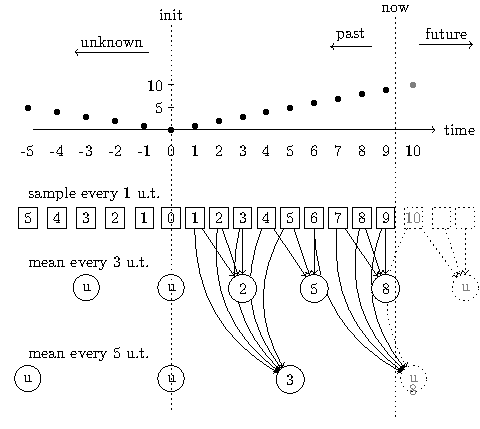
\includegraphics{fig_mtsms_sequence.pdf}
  \caption{Multiresolution snapshot diagram with regular sampling}
  \label{fig:mtsms:sequence}
\end{figure}

At the bottom of Figure~\ref{fig:mtsms:sequence} there is a diagram
that shows how multiresolution works. The first row displays the
signal's sample values that correspond to the above plot. The sampling
frequency is of one unit of time. The second and the third rows show an
actual schema of a multiresolution database. It consists of two
summaries for the time series resolutions. Every summary has a
distinct resolution. The first of the rows computes the mean of the
sampled values every three units. The second computes the mean every
five units. In this example, the aggregation function corresponds to a
statistical mean. The values before \emph{init} are not acquired, and
they are marked as unknown (\emph{u}). Future values are also marked
as unknown \emph{u} until time advances. Therefore, the first summary
for the original signal at time instant \emph{now} corresponds to
values $\{u,u,2,5,8,u\}$.

The multiresolution approach enhances \acro{TSMS} features in several
aspects:

\begin{itemize}

\item Voluminous data. The monitoring systems capture an enormous
  amount of data from sensors. To be able to process these data, their
  volume must be reduced. The multiresolution approach allows to
  select and store only the most interesting segments of data. We
  understand these segments as different resolution views for the same
  time series. The user can configure how these segments are extracted
  and summarised by defining different time steps and
  functions. Multiresolution also facilitates the graphing of huge
  time series. It allows to select the best time range and time step
  that makes the graph fit on the screen. Because we cannot appreciate
  more data on the screen, there is no need to render it.

\item Data validation. The use of monitoring systems to capture data
  is a current practice. However, the nature of these systems has some
  drawbacks that have an impact on the obtained data. Quevedo et
  al.~\cite{quevedo10} note that the main problems arise when the
  monitoring system cannot capture data, producing errors known as
  gaps, or when the monitoring system captures data erroneously.  The
  multiresolution attribute functions are designed to cope well with
  validation, filtering and reconstruction of these unknown data to
  keep a consistent history.

\item Data time regularisation. To monitor with a non-constant
  sampling rate has a side effect that induces irregularities in
  data. According to Kopetz~\cite{kopetz11:realtime} there are two
  main reasons for sampling rate variation: either sampling jitters in
  periodic sampling or non-periodic rates caused by event-based
  sampling.  Multiresolution regularises the time interval while
  processing a time series. As a consequence, every obtained time
  series segment has a regular time resolution. This feature can also
  be used to query the time series using some other resolution. For
  instance, a daily acquired time series can be queried using a yearly
  step.

\item Data summaries. A goal of a database system is to answer the
  user queries about the stored information. The multiresolution
  approach allows a lossy compression storage solution. In some sense,
  it is an online way to compute and store data summaries, i.e. data
  of interest. These stored data summaries allow faster queries of
  voluminous data. However, we should determine the summaries
  organization a priori considering the context where the future
  queries will be issued.

\end{itemize}


%%% Local Variables:
%%% TeX-master: "main"
%%% ispell-local-dictionary: "british"
%%% End:

%  LocalWords:  multiresolution TSMS MTSMS timestamp timestamps equi
%  LocalWords:  SQL NoSQL NewSQL et al metadata Segev Shoshani Dreyer
%  LocalWords:  Calanda Quevedo Kopetz outliers
